\chapter{引言}
本章首先介绍光学模型的基本理论及其物理图像，随后综述阈异常现象及相关研究进展，在此基础上引出本文的研究对象——大形变体系 $^{18}\mathrm{O}+^{152}\mathrm{Sm}$ 的光学势阈异常问题，并阐述本工作的研究目标与科学意义。
\section{光学模型}

自Fernbach等人\cite{fernbach1949scattering}首次将光学模型应用于描述中子在不同靶核上的核散射与核吸收过程以来，该模型在过去七十余年间得到了广泛发展，并在核反应研究中取得了巨大成功，现已成为核物理学中最基本、最常用的反应模型之一。其核心思想在于：入射粒子与靶核相互作用时所表现出的散射、透射及吸收行为，与光波在具有复折射率介质中的传播过程具有高度相似性\cite{feshbach1958optical,hodgson1971nuclear}。因此，人们将描述粒子与原子核相互作用的复势称为光学势（optical potential）。

\subsection{理论基础}

在光学模型建立之前，人们曾尝试采用单纯的实势阱来描述入射粒子与靶核之间的相互作用。然而很快发现，无论势阱参数如何选取，都难以同时解释低能中子核反应实验中观测到的激发函数共振峰以及异常大的吸收截面。为了解释这些现象，Bohr提出了复合核理论。该理论认为，入射粒子首先在核表面受到散射，入射粒子进入核内部后，可与靶核形成统计平衡的复合核态，随后复合核再通过粒子发射、$\gamma$退激发或裂变等方式衰变，从而产生各种反应结果。

由于复合核模型假定入射粒子进入核内后几乎必然被吸收，因此又常被称为强吸收模型。当入射粒子的能量恰好使形成的复合核处于某一准稳定能级附近时，反应截面会在狭窄能区内迅速增大，表现为共振现象，这一机制能够较好解释早期实验中观察到的窄共振结构。

尽管复合核理论成功解释了许多现象，但随着实验精度提高，人们逐渐发现其也存在局限性。随着实验精度提高，人们逐渐发现复合核理论存在局限性。例如，中高能区平滑激发函数以及直接反应过程的普遍存在，都表明入射粒子与靶核之间的相互作用并非总是强吸收的。实验表明，部分入射粒子可以穿过核表面，在未形成复合核的情况下直接与核内核子发生一次或少数几次相互作用，从而产生转移反应、非弹性散射等过程。

这一认识促使人们重新审视核内运动图像。20世纪40年代末，壳模型的成功表明，由于泡利不相容原理的限制，核子在核内与其他核子频繁交换能量和动量的概率远低于自由空间情形，因此每个核子可近似看作在其他核子共同产生的平均势场中独立运动。显然，这一平均场图像同样适用于外来入射粒子。于是，人们开始采用平均场方法描述入射粒子与靶核之间的相互作用，并在其中引入复数势来统一处理弹性散射与非弹性吸收过程。

相互作用势即光学势可写为

\begin{equation}
U(r)=V(r)+iW(r),
\end{equation}

其中，实部势 $V(r)$ 描述吸引性的平均核力作用，决定散射过程中的透射、折射与反射行为；虚部势 $W(r)$ 描述其他反应通道引起的吸收效应，反映入射通量从弹性道向非弹性散射、转移反应、复合核形成及融合等过程的损失。

从物理图像上看，入射粒子在靶核平均复势阱中传播时，其波函数一部分被散射回弹性道，形成势弹性散射或形状弹性散射；另一部分则由于虚部势耦合进入其他开放反应道而被“吸收”。若将入射粒子视为光波，则早期强吸收模型对应于几乎完全吸收入射光的“黑体”；而复数势描述下的原子核则更类似于一种既能散射又能部分吸收的半透明介质，这正是“光学模型”名称的由来。

光学模型提出后得到了持续发展，并已成为核反应研究中最重要的理论工具之一。。20世纪50年代初，人们已能够利用简单的光学势较准确地描述多种核素上的中子散射截面与吸收截面。此后经过不断发展与修正，光学模型逐步形成了一整套系统理论，并成为分析核反应数据、提取核势参数以及研究核反应机制的重要工具。

\subsubsection{唯像的光学模型势}

虽然光学模型的理论框架十分清晰，但光学势的具体形式并不能完全由基本理论直接给出。因此，研究者通常依据核力的短程性质、核结构知识以及微观模型得到的定性结论，预先假定光学势具有某种参数化形式，其中包含若干待定参数，再通过拟合实验测得的弹性散射角分布、总反应截面及其他观测量来确定这些参数。采用这种方法建立的光学势称为唯象光学势（phenomenological optical potential）。

相对运动的有效势通常写为
\[
U_{\mathrm{eff}}(r)=V_C(r)+V_N(r)+V_{\mathrm{cent}}(r)
\]
其中光学势本身通常指
\[
U(r)=V_C(r)+V_N(r)
\]

其中，$V_C(r)$ 为库仑势，$V_N(r)$ 为核势，$V_{\mathrm{cent}}(r)$ 为离心势。在数值计算中，离心势通常已自动包含在径向薛定谔方程中，因此往往无需单独写出。

库仑势 $V_C(r)$ 一般采用电荷均匀分布、半径为 $R_C$ 的带电球模型表示：

\begin{equation}
V_C(r)=
\begin{cases}
\dfrac{Z_p Z_t e^2}{2R_C}\left(3-\dfrac{r^2}{R_C^2}\right), & r<R_C,\\[8pt]
\dfrac{Z_p Z_t e^2}{r}, & r\ge R_C.
\end{cases}
\end{equation}

其中

\begin{equation}
R_C=r_C A^{1/3},
\end{equation}

$r_C$ 为约化库仑半径，通常取 $1.3\ \mathrm{fm}$ 左右。

核势 $V_N(r)$ 一般由中心实部势、虚部吸收势以及自旋轨道耦合势组成：

\begin{equation}
V_N(r)=V(r)+iW(r)+U_{so}(\mathbf{L}\cdot\mathbf{S}).
\end{equation}

其中中心实部势通常写为

\begin{equation}
V(r)=-Vf(r),
\end{equation}

这里 $V$ 为势深度，$f(r)$ 为形状因子。由于核力属于短程相互作用，势阱在核内部通常近似平坦，在核表面区域逐渐下降，并在核外迅速趋近于零。满足上述性质的最常用参数化形式为 Woods-Saxon 势：

\begin{equation}
f(r)=\left[1+\exp\left(\frac{r-r_0(A_p+A_t)^{1/3}}{a_0}\right)\right]^{-1}.
\end{equation}

其中 $r_0$ 为半径参数，$a_0$ 为弥散参数，二者均通过实验拟合确定。

虚部吸收势通常分为体吸收项与表面吸收项：

\begin{equation}
W(r)=-W_V f_V(r)-W_S\left(-4a_s\frac{d}{dr}f_S(r)\right).
\end{equation}

其中 $W_V$ 描述核内部吸收效应，$W_S$ 描述主要发生在核表面的吸收过程。由于表面吸收在核表面附近达到峰值，因此常采用 Woods-Saxon 函数的导数形式表示。

自旋轨道耦合势可写为

\begin{equation}
U_{so}=-(V_{so}+iW_{so})
\left[-\left(\frac{\hbar}{m_\pi c}\right)^2
\frac{1}{r}\frac{d}{dr}f_{so}(r)\right],
\end{equation}

其中 $V_{so}$ 与 $W_{so}$ 分别为实部与虚部自旋轨道强度参数，$\left(\frac{\hbar}{m_\pi c}\right)^2$ 为 $\pi$ 介子康普顿波长的平方。

在重离子反应研究中，为减少自由参数数量，常采用标准 Woods-Saxon 光学势，仅保留中心实部势、体吸收虚部势及库仑势。此时主要可调参数通常为六个，即 $V,r_{0V},a_V,W,r_{0W},a_W$。

\subsubsection{双折叠模型}

唯象光学势虽然能够有效描述实验数据，但其参数往往依赖具体体系与入射能量，缺乏统一的微观基础。为了从更本质的角度理解核势来源，人们进一步发展了微观光学模型。其中最成功、应用最广的方法之一便是双折叠模型（double-folding model）。

折叠模型的基本思想是：两个碰撞核之间的相互作用势，可以看作构成它们的全部核子之间有效核子--核子相互作用的平均结果。也就是说，将核子--核子相互作用对两个碰撞核的物质密度分布进行积分，便可得到核与核之间的平均相互作用势。若同时对弹核与靶核的全部核子坐标进行积分求和，则称为双折叠模型。

其数学形式为

\begin{equation}
V(r)=\int \rho_P(\mathbf{r}_1)\rho_T(\mathbf{r}_2)
v_{12}(\mathbf{r}+\mathbf{r}_2-\mathbf{r}_1)\,
d\mathbf{r}_1 d\mathbf{r}_2,
\end{equation}

其中，$\rho_P(\mathbf{r}_1)$ 与 $\rho_T(\mathbf{r}_2)$ 分别为弹核和靶核的物质密度分布函数，$v_{12}$ 为有效核子--核子相互作用势，$\mathbf{r}$ 为两核质心间距。

在实际应用中，常采用M3Y系列有效相互作用，如 Reid 型或 Paris 型势。为了更真实地反映核介质效应，通常还需引入密度依赖项与能量依赖项，因此有效相互作用写为

\begin{equation}
v(r,\rho,E)=g(E)F(\rho)v_{\mathrm{M3Y}}(r),
\end{equation}

其中 $g(E)$ 描述入射能量依赖性，$F(\rho)$ 描述周围核介质密度对核子间相互作用的修正，$v_{\mathrm{M3Y}}(r)$ 为基本M3Y相互作用势。

双折叠模型在重离子弹性散射、融合反应及近垒核反应研究中得到了广泛应用，并能为唯象光学势参数提供重要约束。由于其积分本质上为六维积分，直接计算较为困难，因此通常借助傅里叶变换将积分由坐标空间转换至动量空间，从而把六维积分化简为二维积分，大幅提高计算效率。

\subsubsection{弹性散射}

弹性散射是研究核相互作用势最直接、最重要的实验手段之一。在弹性散射过程中，入射粒子 $a$ 与靶核 $A$ 的内部量子态保持不变，仅体系相对运动状态发生变化。因此，散射过程所反映的信息主要来自两者之间的相互作用势。

对于在势场 $V$ 中相互作用的两粒子体系，其相对运动波函数满足定态薛定谔方程：

\begin{equation}
\left[-\frac{\hbar^2}{2\mu}\nabla^2+V-E\right]\psi=0,
\end{equation}

其中 $\mu$ 为体系折合质量，$E$ 为体系在质心系中的相对运动能量。

当 $r\rightarrow \infty$ 时，波函数应满足渐近边界条件：

\begin{equation}
\psi(\mathbf{r})\sim e^{ikz}+f(\theta)\frac{e^{ikr}}{r},
\end{equation}

其中第一项 $e^{ikz}$ 为沿 $z$ 方向传播的入射平面波；第二项为向外传播的球面散射波；$f(\theta)$ 为散射振幅，它包含体系动力学的全部散射信息。

根据散射理论，微分截面定义为单位时间内散射到单位立体角中的粒子数与入射流密度之比，因此有

\begin{equation}
\frac{d\sigma}{d\Omega}=|f(\theta)|^2.
\end{equation}

由此可见，实验测得的角分布本质上由散射振幅决定，而散射振幅又是相互作用势的函数。因此，弹性散射微分截面可以视为光学势的泛函。通过对实验角分布数据进行拟合，便可反推出散射体系的光学势参数，从而获得核相互作用的重要信息。这也是光学模型在实验核物理研究中长期占据核心地位的根本原因。
\subsection{光学势的阈异常现象}
20世纪80年代中期，实验发现光学势在库仑势垒附近具有能量依赖性\cite{baeza1984energy,lilley1985evidence}，图~\ref{fig:TA}展示了$^{16}\mathrm{O}$+$^{208}\mathrm{Pb}$体系光学势的特点：当能量降低至库仑势垒以下，虚部势随着非弹性反应道的闭合而急剧减小，从而出现阈值现象；同时实部势在势垒附近呈现出钟罩形的异常增强行为。这一现象由此被称为阈异常\cite{nagarajan1985dispersion,mahaux1986causality,satchler1991heavy,brandan1997interaction}（threshold anomaly，TA）。

\begin{figure}[h]
\centering
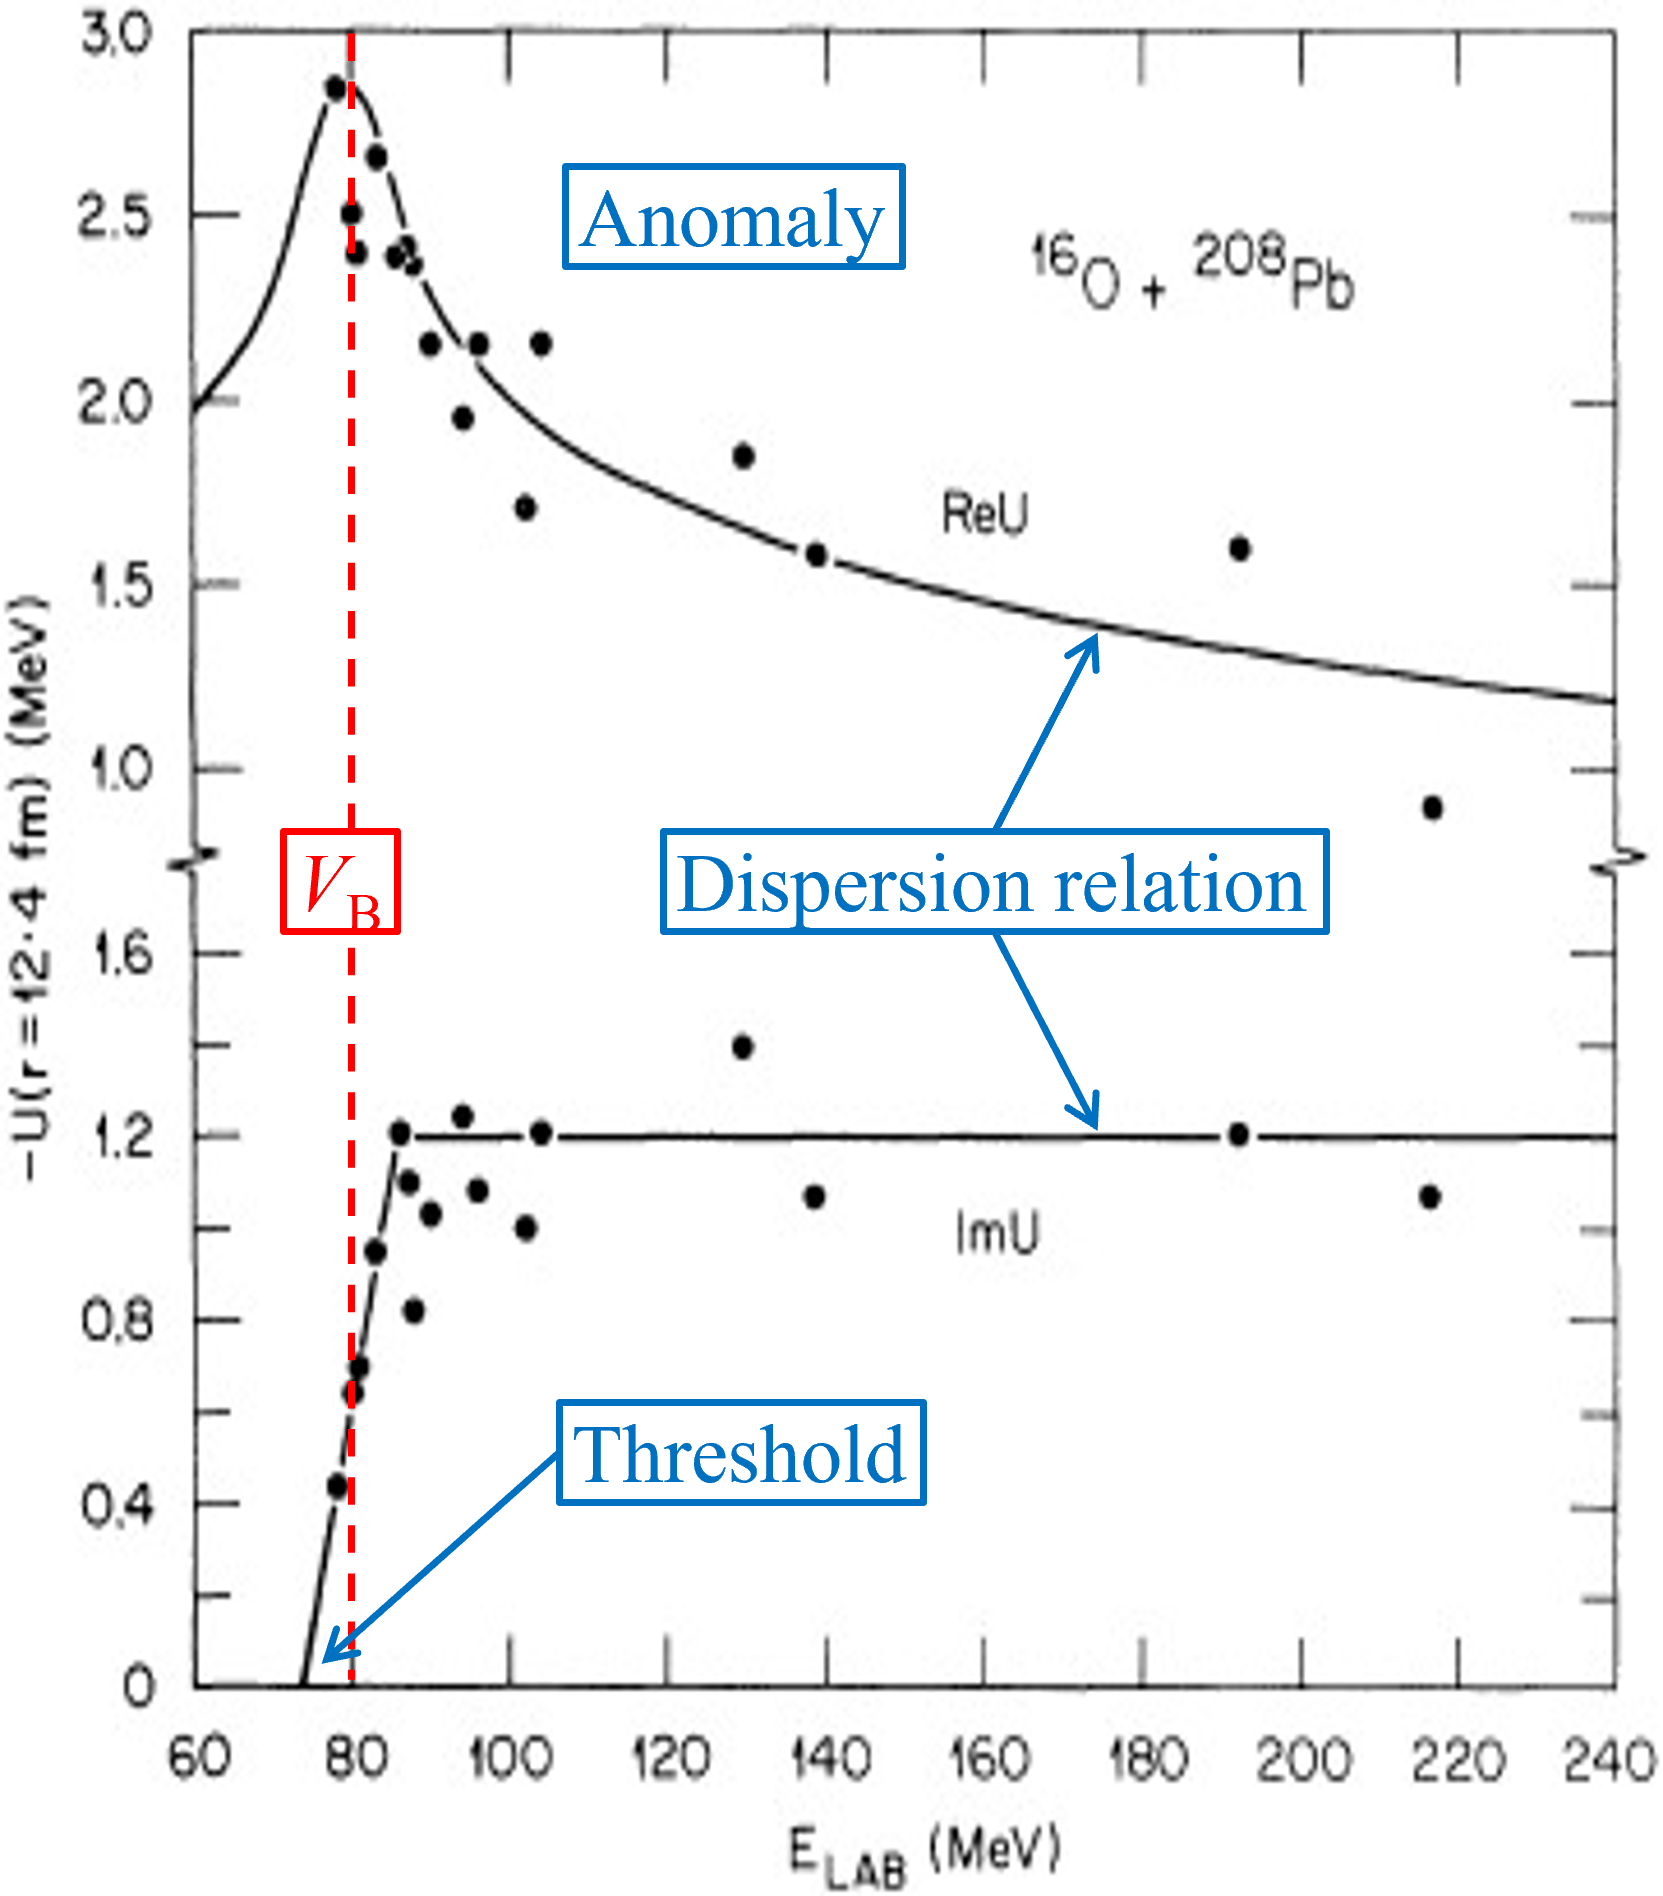
\includegraphics[width=0.7\linewidth]{images/典型的阈异常.png}
\caption{典型的光学势阈异常行为}
\label{fig:TA}
\end{figure}

基于此，光学模型势被表述为
\begin{equation}
U(r;E) = V(r;E) + iW(r;E)
\end{equation}
其中，实部势$V(r;E)$通常可分解为
\begin{equation}
V(r;E) = V_0(r;E) + \Delta V(r;E)
\end{equation}
实部势的第一项源于空间非定域性，通常在大能量范围内呈现缓慢平滑的能量依赖性；第二项称为动力学极化势，由时间非定域性导致，并通过色散关系与虚部势相关联:
\begin{equation}
\Delta V(r;E) = \frac{P}{\pi}\int^\infty_0\frac{W(r;E')}{E'-E}dE'
\label{kk}
\end{equation}
其中P为积分主值。色散关系（一般情况下称为Kramers-Kronig关系）是根据因果律自然得到的结果，描述了介质中的色散效应对波在该介质中传播特性的影响。目前发现大量体系如$^{16}\mathrm{O}$+$^{208}\mathrm{Pb}$\cite{nagarajan1985dispersion}、$^{19}\mathrm{F}$+$^{208}\mathrm{Pb}$\cite{lin2001threshold}、$^{7}\mathrm{Li}$+$^{208}\mathrm{Pb}$\cite{keeley1994optical}、$^{16}\mathrm{O}$+$^{60}\mathrm{Ni}$\cite{fulton1985energy}、$^{32}\mathrm{S}$+$^{40}\mathrm{Ca}$\cite{diaz1989threshold}等，其光学势的实部虚部势深度整体上都满足色散关系，普遍有阈异常的现象。

由于光学势参数是从角分布数据上抽取得到的，所以一个体系角分布的行为会与其阈异常的行为相关联。能量接近库仑势垒时，弹性散射角分布属于典型的Fresnel 散射类型。
图~\ref{fig:3.3} 显示了 $^{16}\mathrm{O}$ 与不同靶核弹性散射的角分布\cite{F1973Elastic}。总体上看，它们有着共同的特征：
\begin{enumerate}
    \item 以 $\mathrm{d}\sigma_{\mathrm{el}}/\mathrm{d}\sigma_{\mathrm{Ru}}$ 形式表达。前角比值 $\cong 1$，基本上是卢瑟福散射；后角比值 $< 1$，减小的部分代表被吸收的成份。
    \item 前角（明区）有明显的明暗条纹，由库仑散射与核散射相干叠加而成，库仑散射为主，故称库仑虹（Coulomb rainbow）；后角（暗区）成对数下降趋势，有明显的边界，核的强吸收特性明显。
    \item $1/4$ 点诀窍（Quarter-point recipe）\ref{fig:3.4}：如图~\ref{fig:3.4}，在 $\mathrm{d}\sigma_{\mathrm{el}}/\mathrm{d}\sigma_{\mathrm{Ru}} = 1/4$ 处，对应的角度为擦边角：$\theta_{\mathrm{gr}} = \theta_{1/4}$；对应的距离为擦边距离（假设沿库仑径迹运动）：
    \[
    R_{\mathrm{gr}} = a\left(1 + \csc(\theta_{1/4}/2)\right)
    \]
    所对应角动量为擦边角动量：
    \[
    L_{\mathrm{gr}} = \eta \cot(\theta_{1/4}/2)
    \]
    在强吸收模型中，$R_{\mathrm{gr}}$ 即为强吸收半径 $R_{\mathrm{sa}}$（参见§1.6）。擦边距离的物理定义为：在该距离处，散射波或吸收波的振幅为 $1/2$，即 $\mathcal{F}(\theta_{1/4}) = 1/2$；这样，
    \[
    \mathrm{d}\sigma_{\mathrm{el}}/\mathrm{d}\sigma_{\mathrm{Ru}} = |\mathcal{F}(\theta_{1/4})|^2 = 1/4.
    \]
\end{enumerate}
\begin{figure}[htbp]
\centering
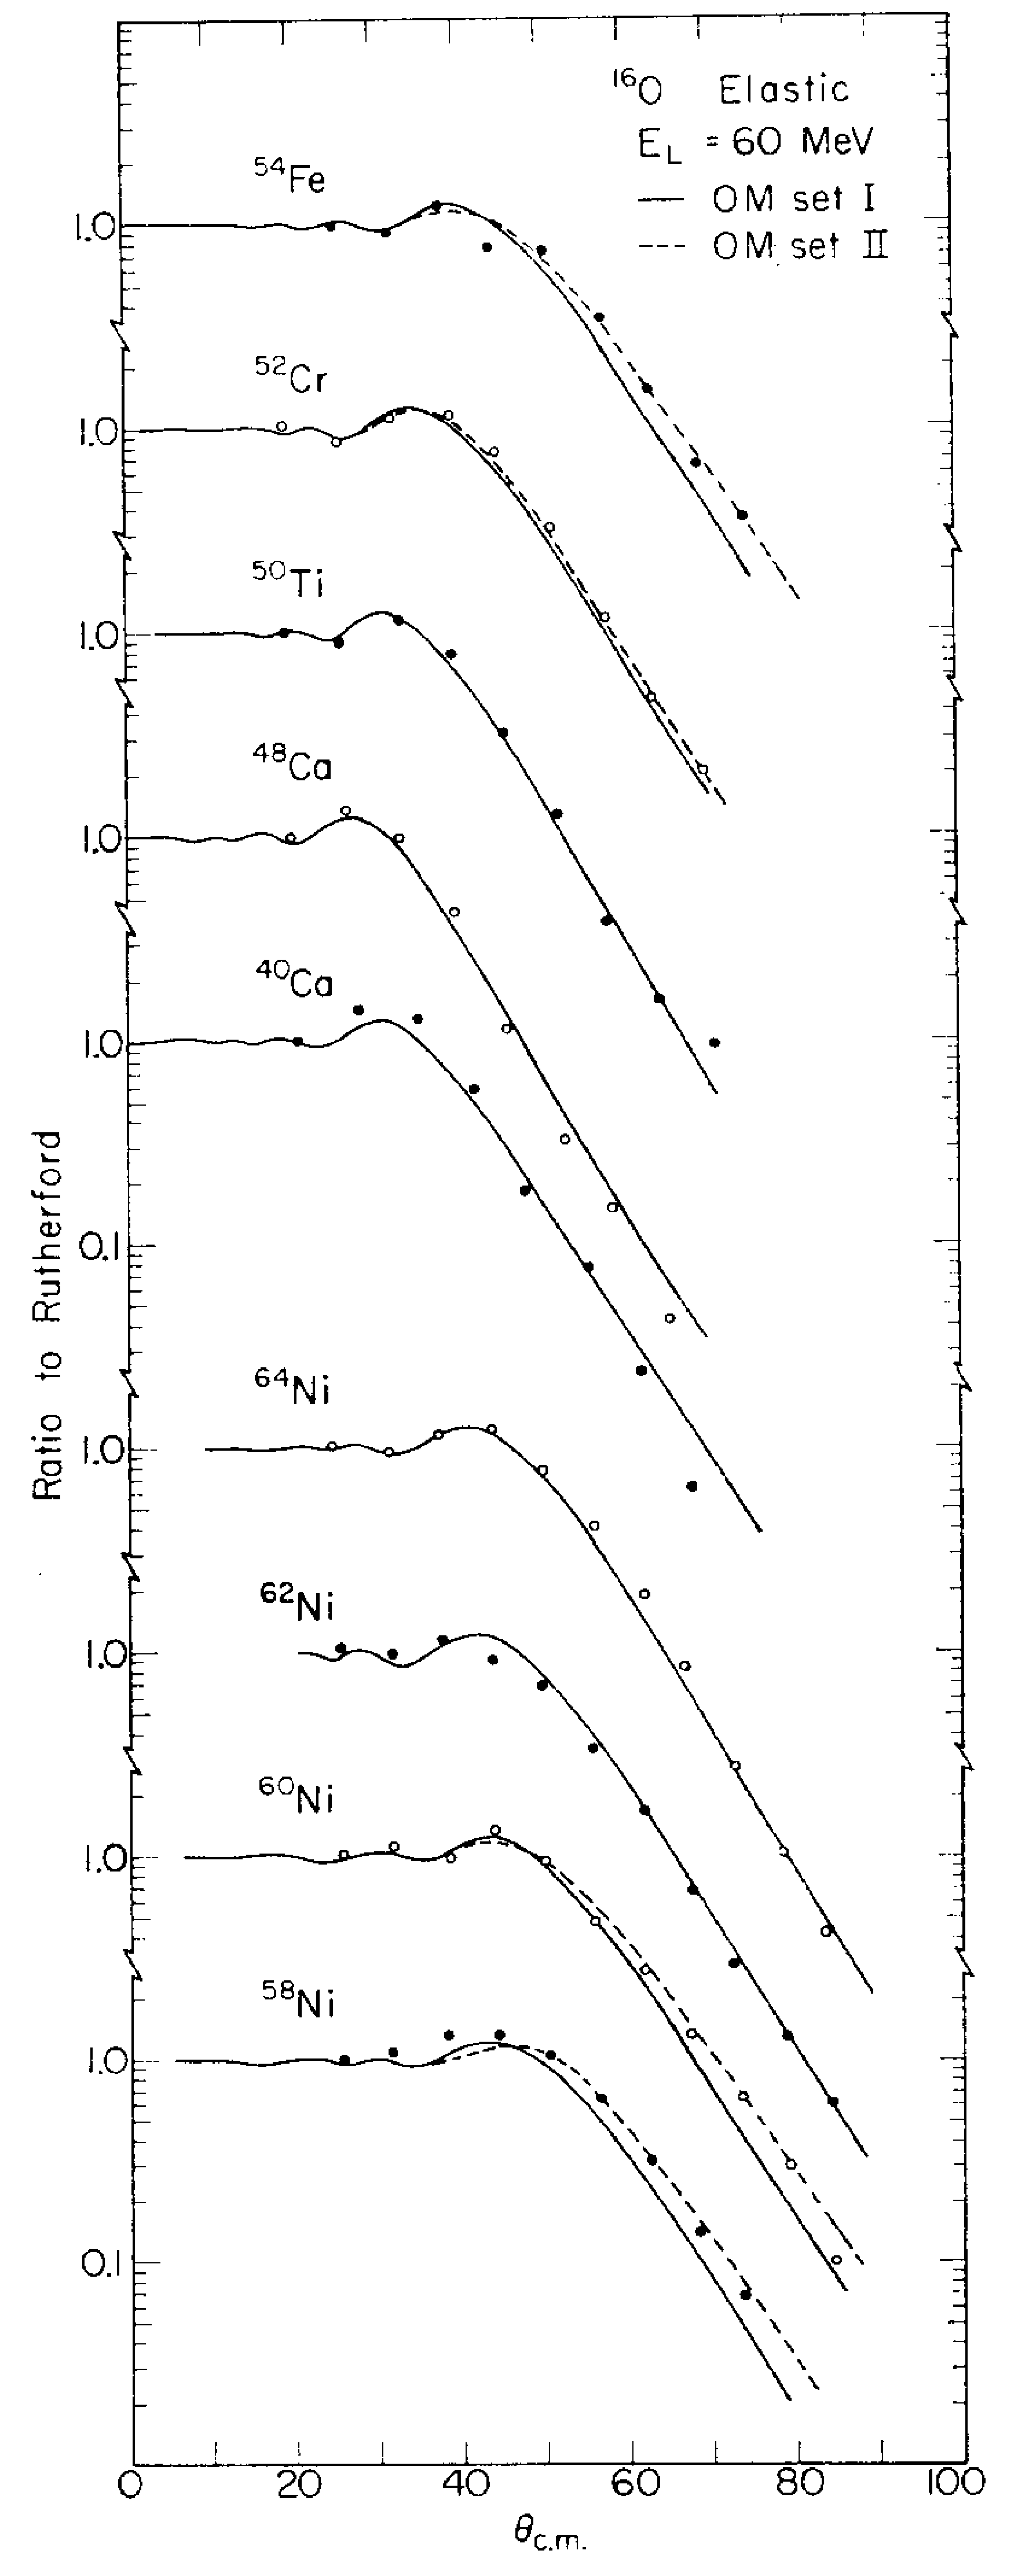
\includegraphics[width=0.45\linewidth]{images/becchetti1973.pdf}
\caption{典型的弹性散射角分布}
\label{fig:3.3}
\end{figure}


\begin{figure}[htbp]
\centering
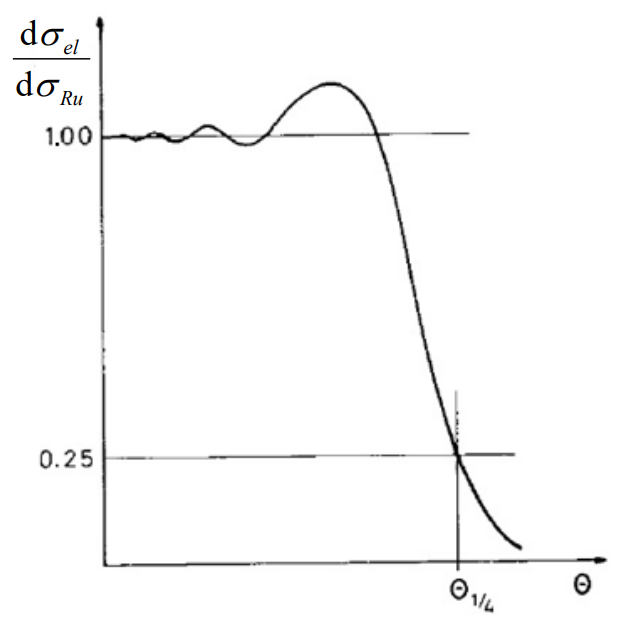
\includegraphics[width=0.6\linewidth]{images/14诀窍.png}
\caption{Quarter-point 示意图}
\label{fig:3.4}
\end{figure}


\section{阈异常现象的研究现状}
% 
\subsection{弱束缚体系}


相较于 $^{16}\mathrm{O}$+$^{208}\mathrm{Pb}$ 这类由球形双幻核组成的紧束缚体系，弱束缚核由于其特殊的结构以及动力学性质，其近垒能区光学势可能呈现出不同的能量依赖行为\cite{hussein2006new,keeley2007fusion}。例如，对于稳定弱束缚核 $^{6}\mathrm{Li}$ 参与的反应体系，如 $^{6}\mathrm{Li}$+$^{28}\mathrm{Si}$\cite{pakou2004elastic}、$^{64}\mathrm{Ni}$\cite{biswas2008study}、$^{80}\mathrm{Se}$\cite{fimiani2012elastic}、$^{138}\mathrm{Ba}$\cite{maciel1999influence}、$^{144}\mathrm{Sm}$\cite{figueira2010energy} 和 $^{208}\mathrm{Pb}$\cite{keeley1994optical}等，实验普遍发现光学势虚部在入射能量降低时反而出现增强。Hussein等人将这种情况称为“破裂阈异常”（Breakup threshold anomaly，BTA）\cite{hussein2006new}，认为这类体系不满足色散关系的原因可能是体系易于破裂，导致入射道通量向连续态通道的大量流失，从而使光学势虚部在势垒附近呈现出异常增强的趋势。同样，对于弱束缚核体系$^{9}\mathrm{Be}$+$^{208}\mathrm{Pb}$、$^{209}\mathrm{Bi}$
\cite{gomez2015energy}，光学势也表示出了明显的破裂阈异常行为。但是，对于与$^{6}\mathrm{Li}$+$^{208}\mathrm{Pb}$非常相似的$^{7}\mathrm{Li}$+$^{208}\mathrm{Pb}$体系，其光学势却表现出了与一般情况较为类似的阈异常现象\cite{黄志杰2024近库仑势垒能区}。图\ref{fig:76Lia},\ref{fig:76Lib}展示了$^{7,6}\mathrm{Li}$+$^{208}\mathrm{Pb}$体系的角分布以及光学势的具体行为。从角分布的数据中也可以看到$^{7}\mathrm{Li}$的角分布的库仑虹要更为显著。考虑到$^{7}\mathrm{Li}$（$S_{\alpha}(^7\mathrm{Li})=2.467~MeV$）与$^{6}\mathrm{Li}$（$S_{\alpha}(^6\mathrm{Li})=1.474~MeV$）破裂阈的差异似乎也不足以解释其光学势完全不同的表现，所以在弱束缚核体系上观察到的光学势不满足色散关系的现象也许不应当完全归因于破裂。
综上，弱束缚体系中阈异常行为并未表现出统一规律，其能量依赖特征可能受到破裂阈、转移通道耦合及核结构等多因素共同影响。
\begin{figure}[htbp]
\centering
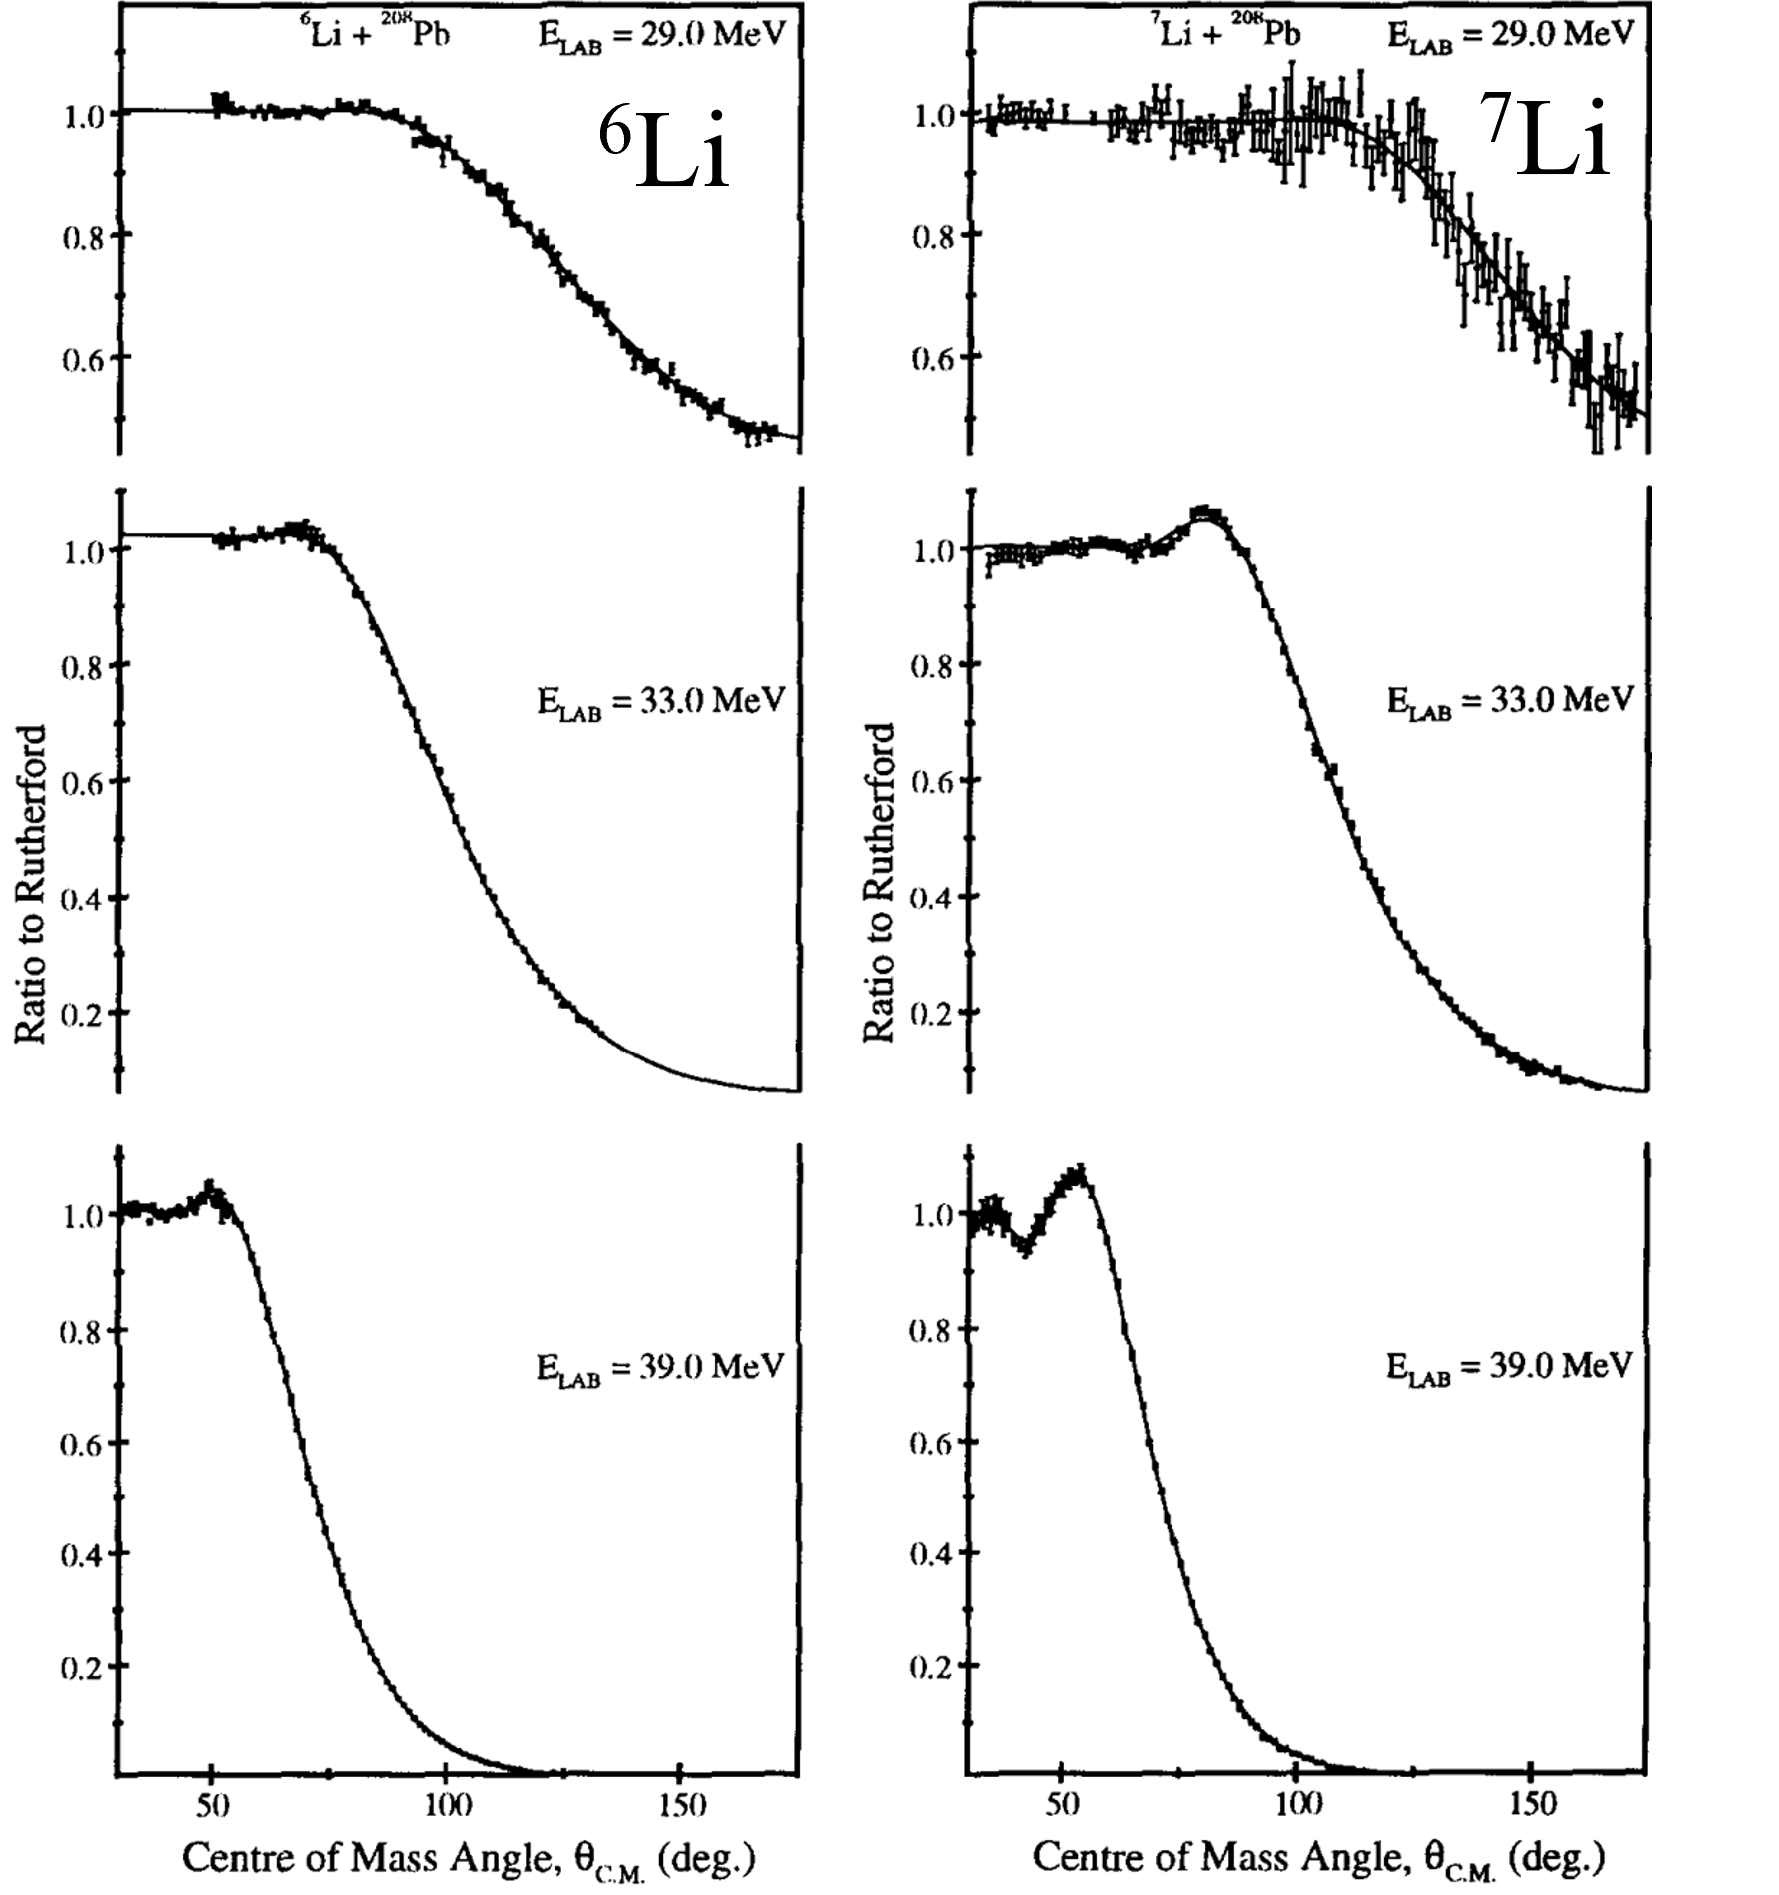
\includegraphics[width=0.7\linewidth]{images/7,6Li角分布.png}
\caption{$^{7,6}\mathrm{Li}$+$^{208}\mathrm{Pb}$体系的角分布示意图}
\label{fig:76Lia}
\end{figure}

\begin{figure}[htbp]
\centering
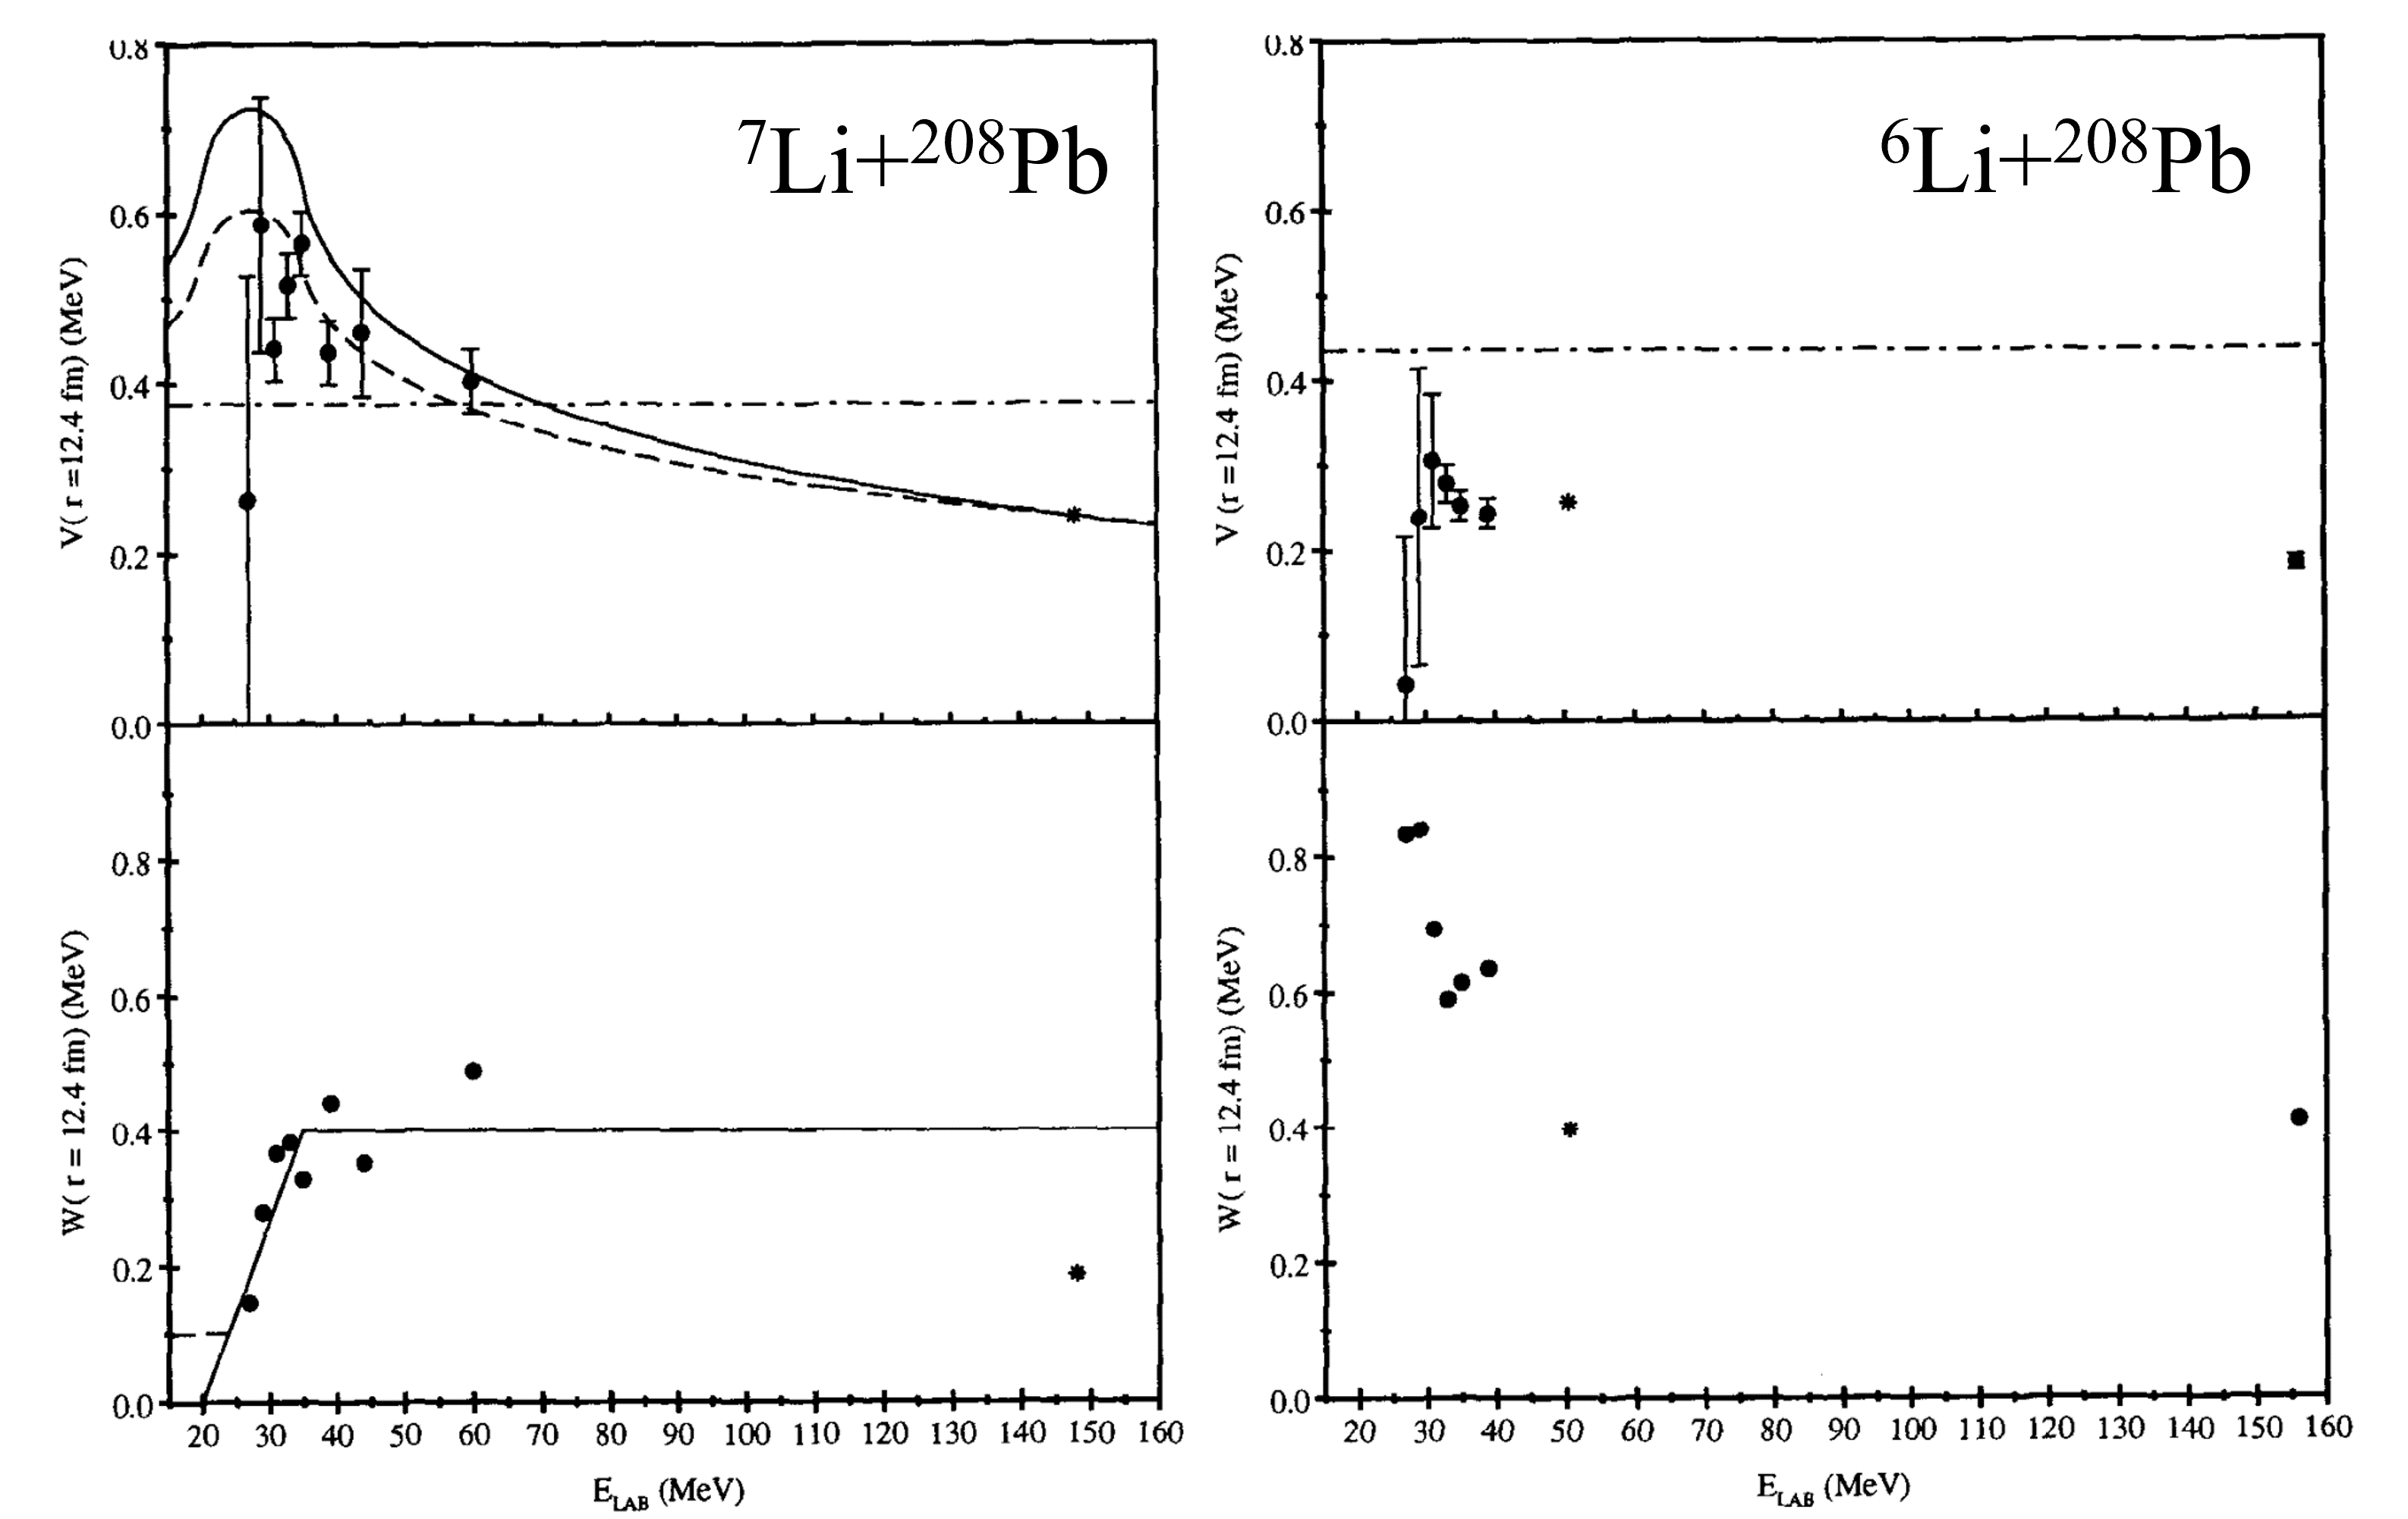
\includegraphics[width=1\linewidth]{images/7,6Li光学势.png}
\caption{$^{7,6}\mathrm{Li}$+$^{208}\mathrm{Pb}$体系的光学势示意图}
\label{fig:76Lib}
\end{figure}


\subsection{晕核体系}
除了弱束缚体系光学势出现了异常行为，从图\ref{fig:11Li},\ref{fig:6Hea}可见，在晕核体系如$^{11}\mathrm{Li}$+$^{208}\mathrm{Pb}$\cite{cubero2012halo}、$^{6}\mathrm{He}$+$^{209}\mathrm{Bi}$\cite{yang2014optical}的弹性散射角分布数据中还观察到了强烈的库仑虹抑制，这是破裂连续态强耦合导致入射道通量大量流失的直接表现。同时，图\ref{fig:6Heb}中可以看到$^{6}\mathrm{He}$+$^{209}\mathrm{Bi}$体系的光学势也被发现不满足色散关系。考虑到$^{11}\mathrm{Li}$（$S_{2\mathrm{n}}(^{11}\mathrm{Li})=0.369~MeV$）与$^{6}\mathrm{He}$（$S_{2\mathrm{n}}(^6\mathrm{He})=0.975~MeV$）的破裂阈要比前面的弱束缚核更低，这些体系的破裂阈与库仑虹抑制以及阈异常之间的关系值得更深入的调查。
因此，晕核体系为研究连续态耦合对光学势能量依赖性的影响提供了理想对象。
\begin{figure}[htbp]
\centering
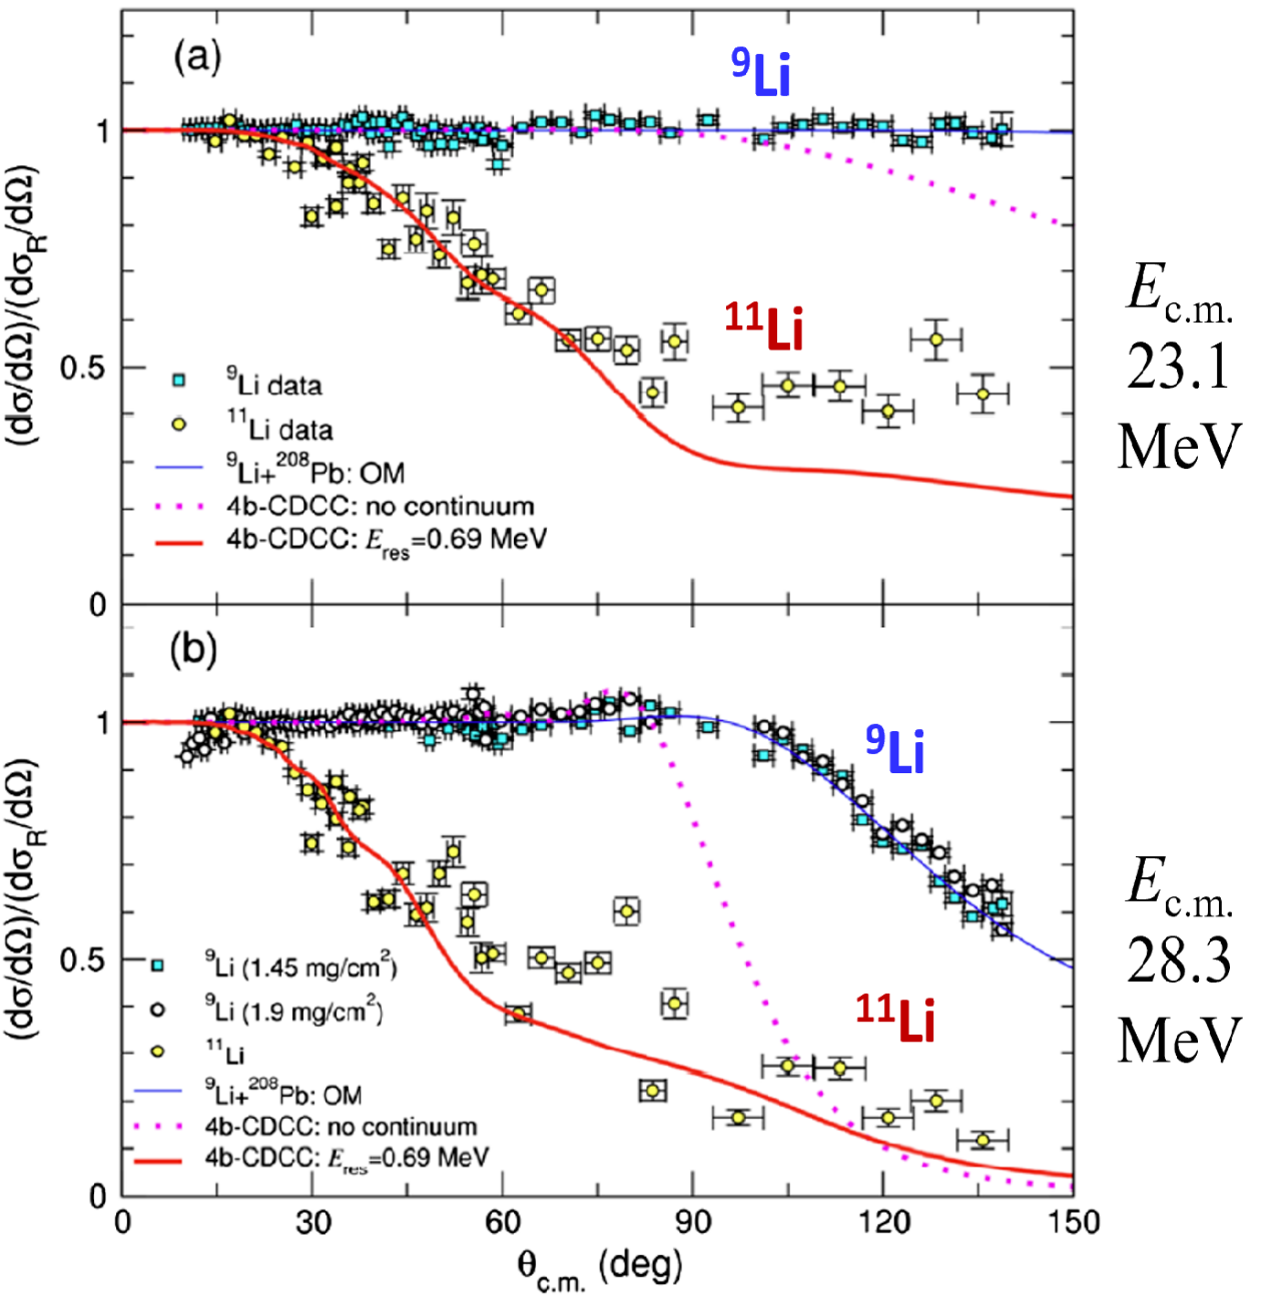
\includegraphics[width=0.7\linewidth]{images/11Li.png}
\caption{$^{11}\mathrm{Li}$+$^{208}\mathrm{Pb}$体系的角分布示意图}
\label{fig:11Li}
\end{figure}

\begin{figure}[htbp]
\centering
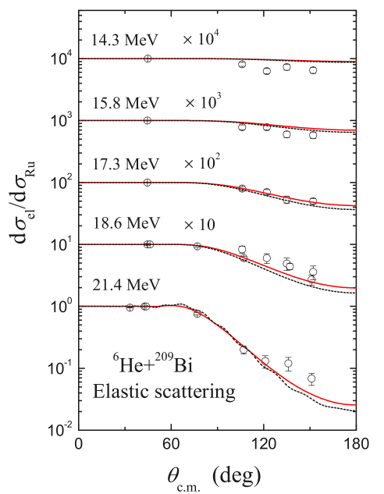
\includegraphics[width=0.6\linewidth]{images/6He角分布.png}
\caption{$^{6}\mathrm{He}$+$^{208}\mathrm{Bi}$体系的光学势示意图}
\label{fig:6Hea}
\end{figure}

\begin{figure}[htbp]
\centering
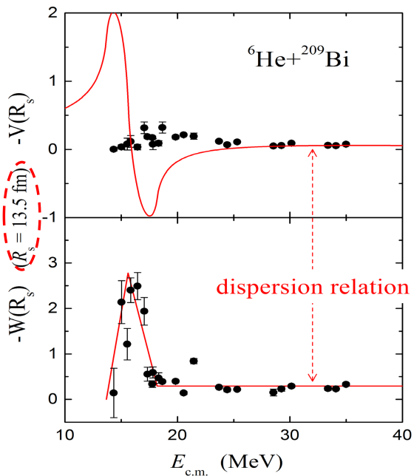
\includegraphics[width=0.6\linewidth]{images/6He光学势.png}
\caption{$^{6}\mathrm{H}$+$^{209}\mathrm{Bi}$体系的光学势示意图}
\label{fig:6Heb}
\end{figure}

\subsection{大形变体系}
另一方面，在大形变核体系也观察到了库仑虹抑制的现象。例如$^{154}\mathrm{Sm}$（$\beta_2$=0.34）或 $^{184}\mathrm{W}$（$\beta_2$=0.25）这样的核具有较大的四极形变参数，其第一激发态能量分别仅为 82~keV 和 110~keV，因此在碰撞过程中极易被激发，非弹激发截面因此显著增大。这种强烈的耦合效应同样会导致入射道通量的大量损失\cite{love1977dynamic}。如图\ref{fig:184W}所示，在 $^{18}\mathrm{O}$+$^{184}\mathrm{W}$ 的弹性散射实验中\cite{thorn1977effect}观察到的库仑虹抑制现象，与在晕核体系中由于破裂连续态强耦合而导致库仑虹被压低的实验现象高度相似\cite{yang2014optical}。图\ref{fig:16OSm}中$\mathrm{Sm}$的各个同位素的角分布同样具有这样的特点，而且可以明显地看到随着形变程度的变化，库仑虹抑制的强度也随之发生变化，那么其光学势的行为也有很有可能进行着逐步的变化。

\begin{figure}[htbp]
\centering
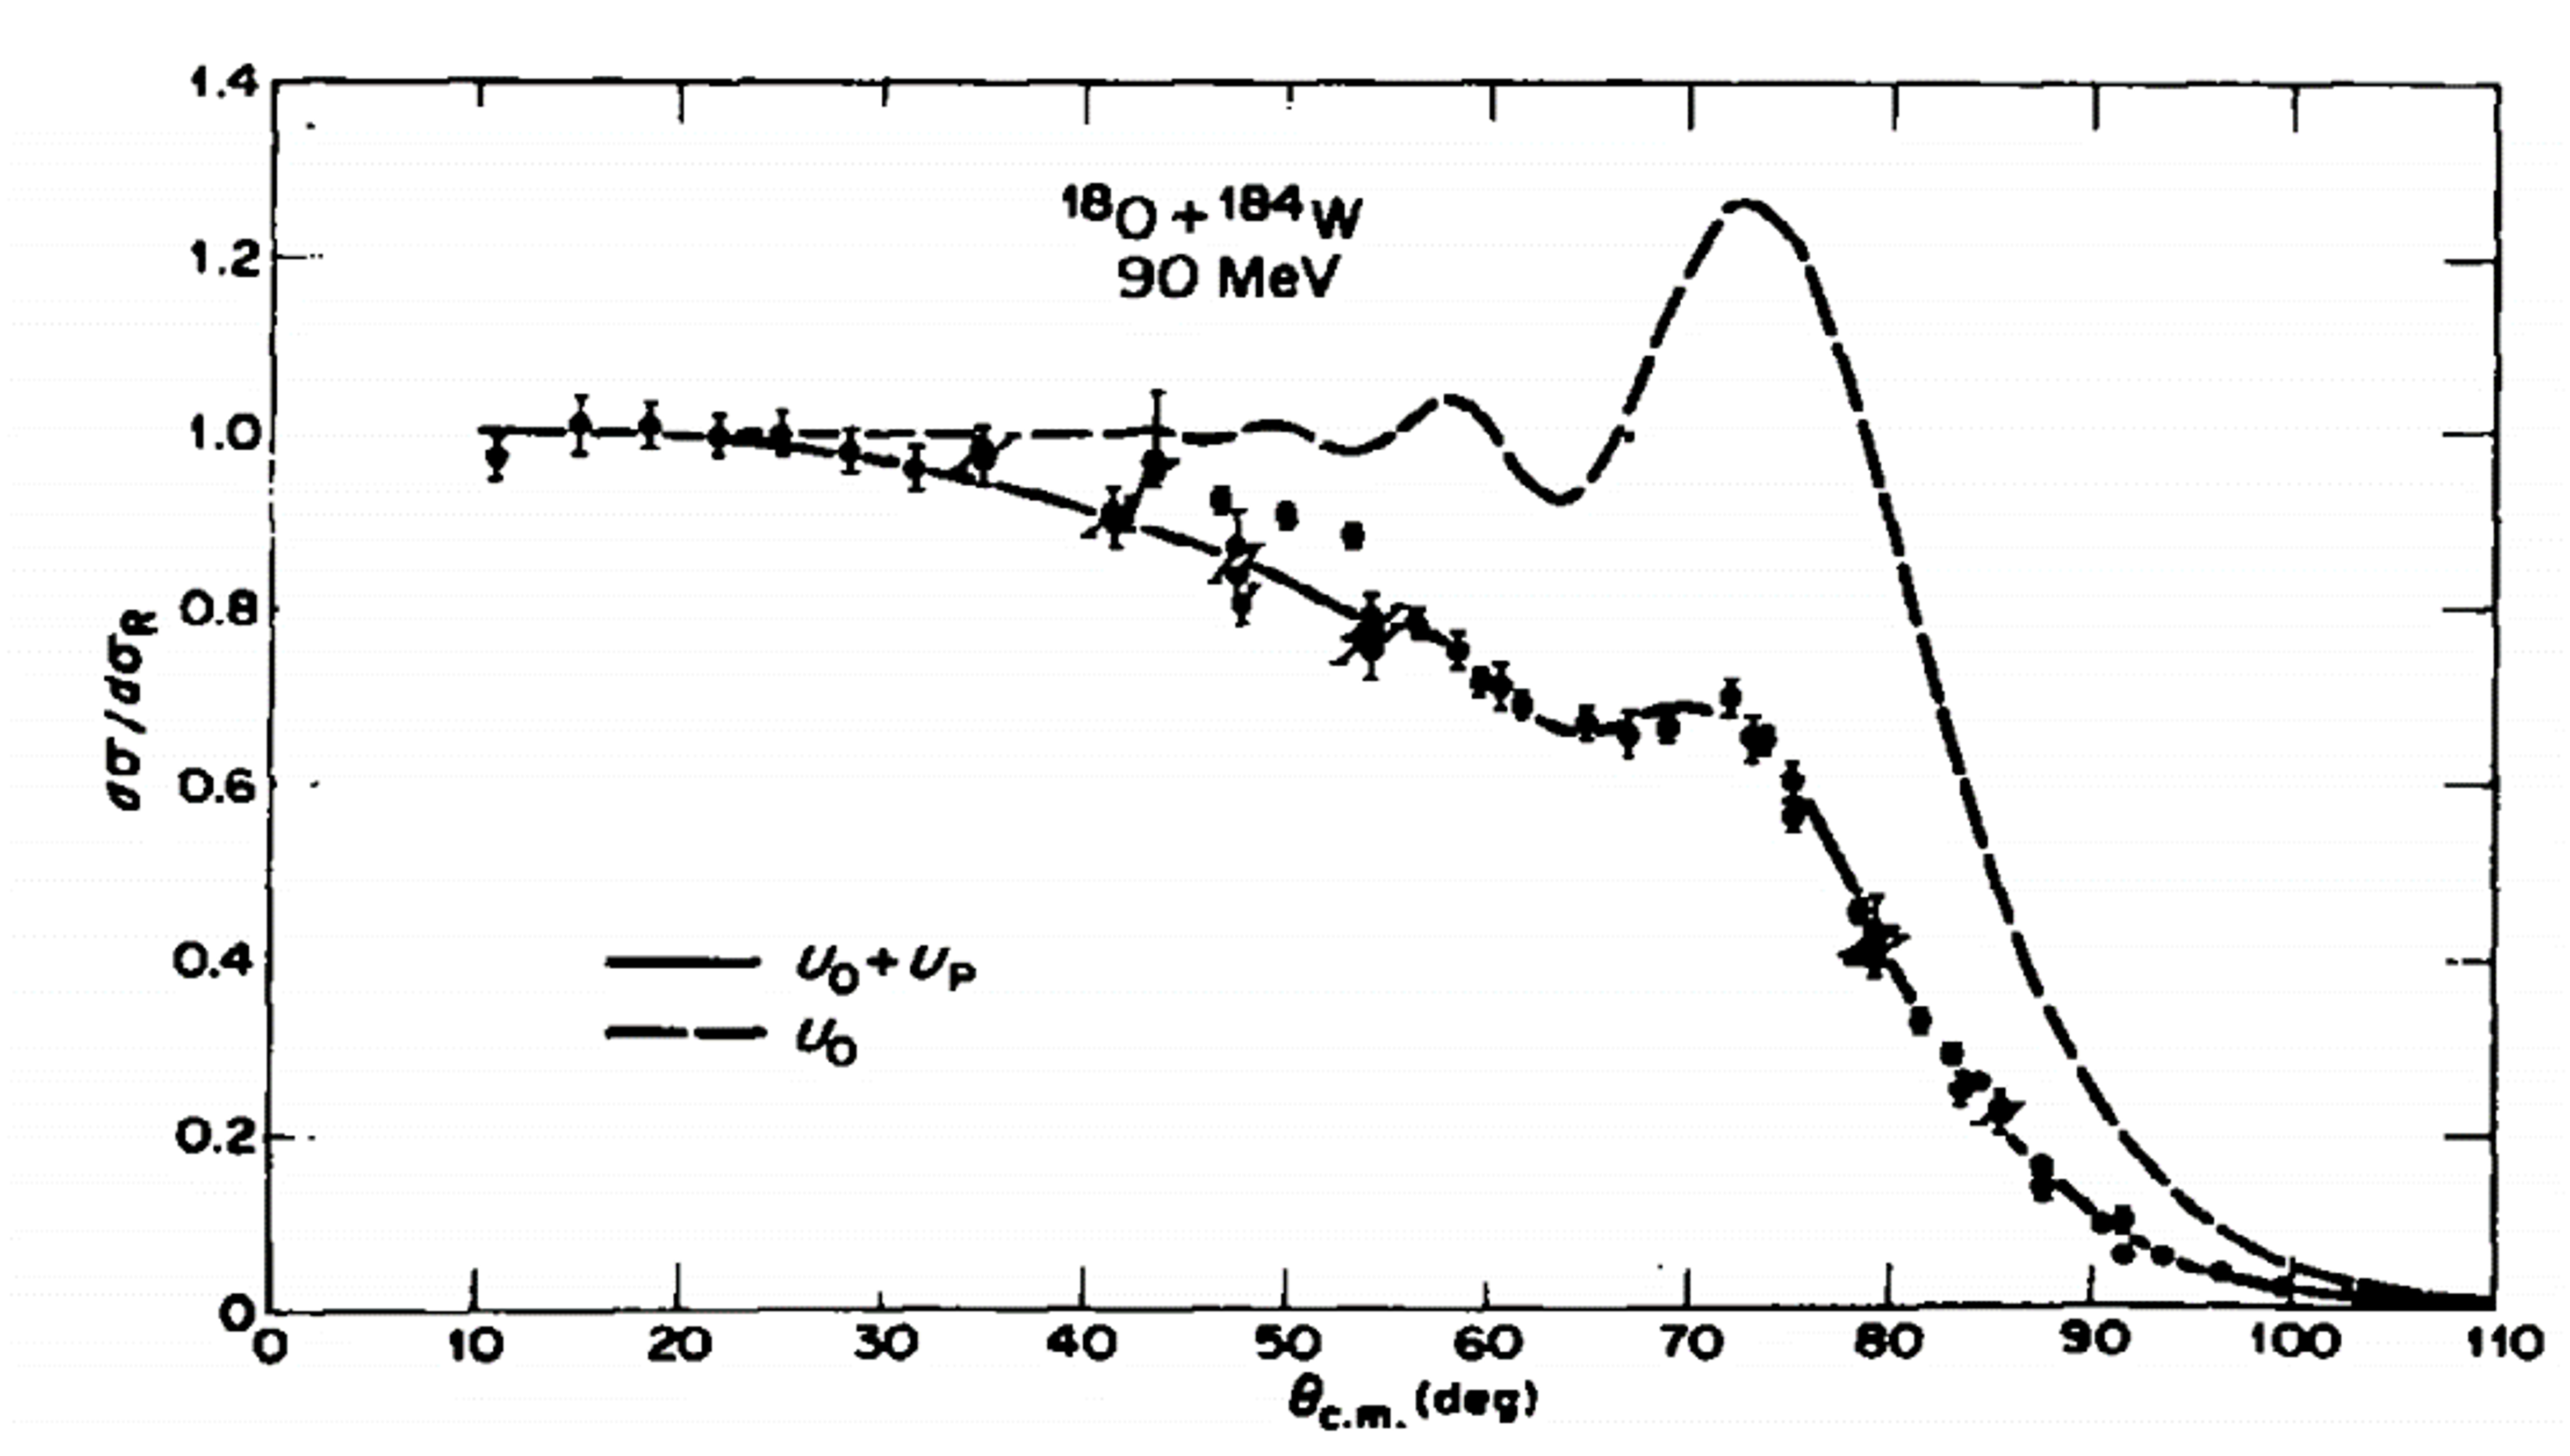
\includegraphics[width=0.8\linewidth]{images/184W.png}
\caption{$^{18}\mathrm{O}$+$^{184}\mathrm{W}$体系的角分布示意图}
\label{fig:184W}
\end{figure}

\begin{figure}[htbp]
\centering
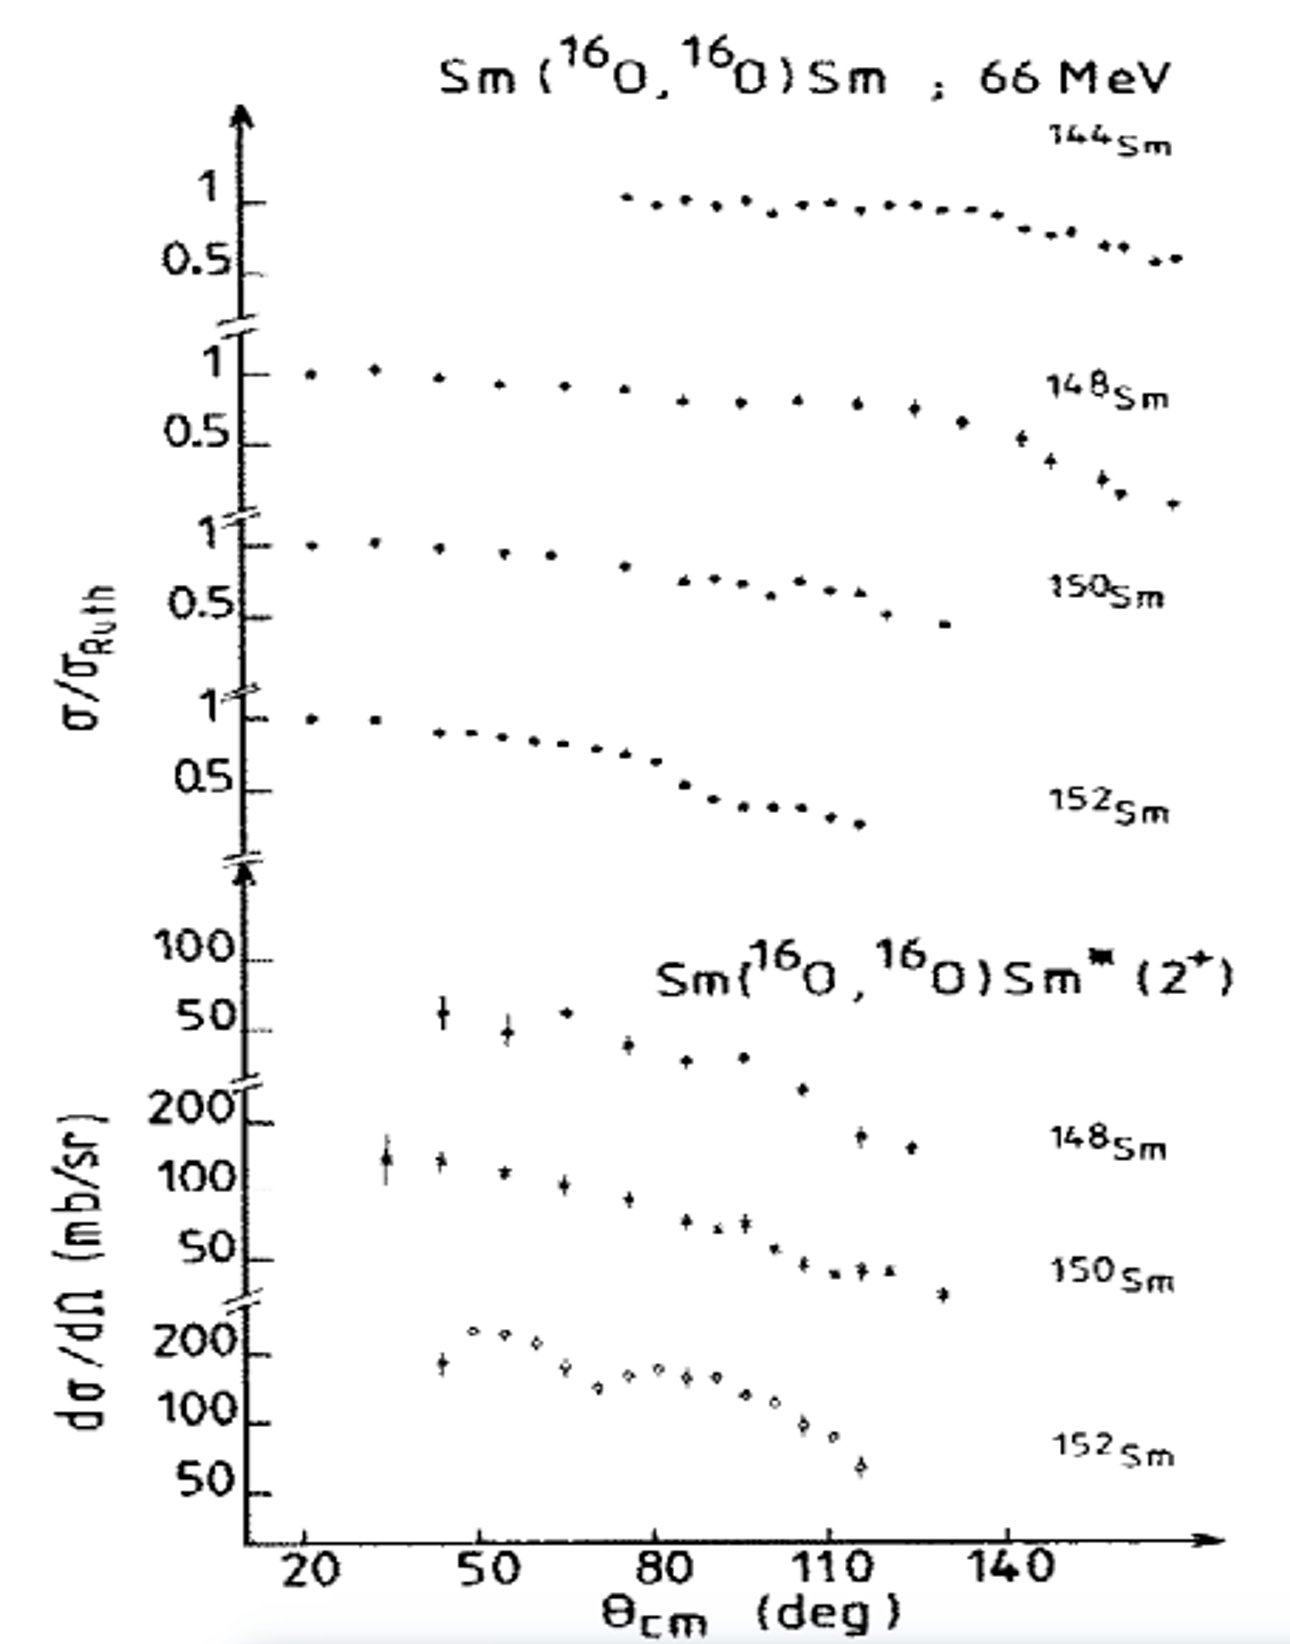
\includegraphics[width=0.6\linewidth]{images/16OSm.png}
\caption{$^{16}\mathrm{O}$+$^{144,148,150,152}\mathrm{Sm}$体系的角分布示意图}
\label{fig:16OSm}
\end{figure}

因此，体系光学势的实部与虚部不满足色散关系可能并不仅仅与破裂有关，更普遍的因素应该是强吸收效应（破裂、转移、非弹激发等），因此“反常阈异常”（Abnormal Threshold Anomaly，ATA）可能是对这种现象更通用的描述。通过系统研究大形变核体系光学势随能量变化的行为，一方面可以有助于确认角分布中的库仑虹抑制现象与光学势中的反常阈异常现象的关联，另一方面可以在弱束缚体系和大形变体系这两类完全不同的体系间一起讨论反常阈异常现象，从而更深入地理解强吸收效应对相互作用势的影响机制，为阐明光学势反常行为提供重要的线索。

目前，与此相关的实验研究仍然十分有限。$^{18}\mathrm{O}$+$^{184}\mathrm{W}$体系的实验仅在单一能点上测量了散射数据\cite{thorn1977effect}；而 $^{16}\mathrm{O}$+$^{152,150,148,144}\mathrm{Sm}$ 体系的实验虽然在多个能量点上测量了弹性散射角分布，但未能从实验数据中可靠地提取光学势参数，从而给出光学势的能量相依性\cite{talon1981coulomb}。这可能与实验统计精度不足、测量能区范围有限、角度覆盖不完整，或相关理论分析方法尚不完善等因素有关。因此，大形变核体系光学势的能量依赖特性仍有待进一步深入研究。
然而，大形变体系相关实验数据仍十分有限，其是否存在系统性的反常阈异常行为尚缺乏直接证据。
\section{论文的主题和意义}
经过多年对光学势阈异常现象的研究，晕核体系与大形变体系的光学势行为已成为低能核物理领域最新、最受关注的研究目标之一，同时这两类体系的实验难度也最高。
对于晕核体系，直接测量其弹性散射角分布需要高流强的放射性束流，这对全球各个核物理设施而言都是极大的挑战。目前虽有尝试通过转移反应来获取晕核体系的角分布，但过程仍十分复杂且成本高昂。
对于大形变体系，则需要极高的能量或动量分辨能力才能实现弹性散射角分布的测量。这要求从束流、制靶到探测体系的每一个环节都精确把控，才能达成目标。
基于上述研究背景，本文选择大形变体系
$^{18}\mathrm O+^{152}\mathrm{Sm}$
作为研究对象，利用Q3D磁谱仪开展近垒能区弹性散射实验，并系统分析其光学势参数随能量的变化规律。

本工作的主要意义体现在以下几个方面：

（1）获得该体系首批高精度、多能点、宽角域弹性散射角分布数据；

（2）提取大形变体系近垒区光学势的能量依赖特征，了解其阈异常行为，检验其光学势是否满足色散关系；

（3）为理解强耦合吸收过程（非弹激发、转移等）对光学势的影响机制提供新的实验依据；

（4）为发展适用于强耦合体系的光学模型参数化形式提供参考。

本论文的内容是这样布局的：
第一章，引言部分。作为全文的开篇章节，本章主要起到提出问题、说明背景和明确研究目标的作用。通过梳理本课题相关理论基础与国内外研究进展，指出当前研究中尚待解决的关键问题与发展趋势，在此基础上引出本文的研究对象、研究思路及主要内容，为后续实验方法、数据分析和结果讨论奠定理论依据与研究背景。
第二章，实验内容部分。作为全文研究工作的基础章节，本章主要起到说明实验实现路径、论证数据来源可靠性以及交代后续分析依据的作用。围绕 $^{18}\mathrm O+^{152}\mathrm{Sm}$ 体系近库仑势垒能区弹性散射测量这一目标，系统介绍实验方案的设计思路、实验装置与探测体系的组成、关键运行参数及实际测量流程，并对动量刻度、立体角刻度及数据获取方法进行说明。通过本章内容，读者能够了解实验数据的获取过程及质量控制方式，为后续角分布提取、光学模型分析和物理结果讨论提供必要的实验依据。
第三章，主要介绍实验方案的选择，实验可行性分析，实验的布局，以及实验中
所涉及的探测器、电子学线路和气路系统；
第四章，实验数据的处理，介绍了实验刻度以及对弹性散射和转移反应的实验数
据的分析和处理，得到弹散和转移反应的角分布；

% 最后回到这里让ai生成一个论文布局
